% Created by tikzDevice version 0.12.6 on 2026-08-03 03:41:03
% !TEX encoding = UTF-8 Unicode
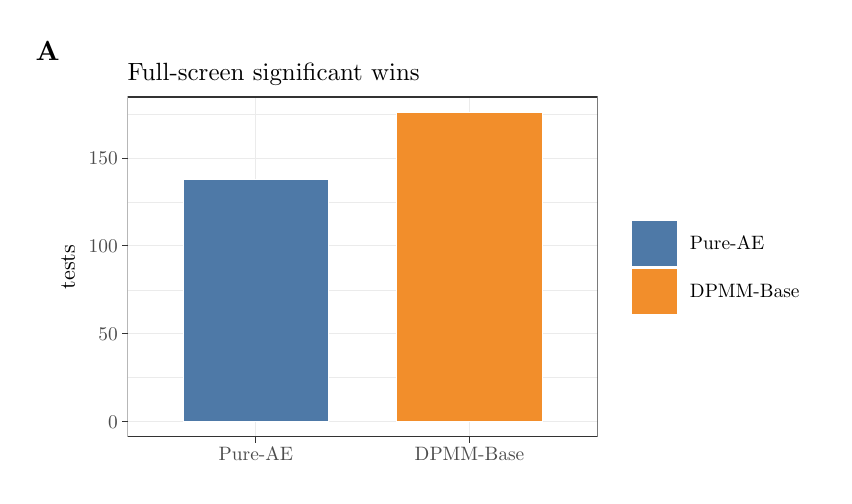
\begin{tikzpicture}[x=1pt,y=1pt]
\definecolor{fillColor}{RGB}{255,255,255}
\path[use as bounding box,fill=fillColor,fill opacity=0.00] (0,0) rectangle (287.75,161.83);
\begin{scope}
\path[clip] (  0.85,  1.74) rectangle (286.90,160.09);
\definecolor{drawColor}{RGB}{255,255,255}
\definecolor{fillColor}{RGB}{255,255,255}

\path[draw=drawColor,line width= 0.4pt,line join=round,line cap=round,fill=fillColor] (  0.85,  1.74) rectangle (286.90,160.09);
\end{scope}
\begin{scope}
\path[clip] ( 36.14, 13.93) rectangle (205.97,136.79);
\definecolor{fillColor}{RGB}{255,255,255}

\path[fill=fillColor] ( 36.14, 13.93) rectangle (205.97,136.79);
\definecolor{drawColor}{gray}{0.92}

\path[draw=drawColor,line width= 0.2pt,line join=round] ( 36.14, 35.38) --
	(205.97, 35.38);

\path[draw=drawColor,line width= 0.2pt,line join=round] ( 36.14, 67.11) --
	(205.97, 67.11);

\path[draw=drawColor,line width= 0.2pt,line join=round] ( 36.14, 98.84) --
	(205.97, 98.84);

\path[draw=drawColor,line width= 0.2pt,line join=round] ( 36.14,130.57) --
	(205.97,130.57);

\path[draw=drawColor,line width= 0.4pt,line join=round] ( 36.14, 19.52) --
	(205.97, 19.52);

\path[draw=drawColor,line width= 0.4pt,line join=round] ( 36.14, 51.25) --
	(205.97, 51.25);

\path[draw=drawColor,line width= 0.4pt,line join=round] ( 36.14, 82.98) --
	(205.97, 82.98);

\path[draw=drawColor,line width= 0.4pt,line join=round] ( 36.14,114.71) --
	(205.97,114.71);

\path[draw=drawColor,line width= 0.4pt,line join=round] ( 82.46, 13.93) --
	( 82.46,136.79);

\path[draw=drawColor,line width= 0.4pt,line join=round] (159.66, 13.93) --
	(159.66,136.79);
\definecolor{drawColor}{RGB}{255,255,255}
\definecolor{fillColor}{RGB}{242,142,43}

\path[draw=drawColor,line width= 0.3pt,fill=fillColor] (133.41, 19.52) rectangle (185.90,131.21);
\definecolor{fillColor}{RGB}{78,121,167}

\path[draw=drawColor,line width= 0.3pt,fill=fillColor] ( 56.21, 19.52) rectangle (108.70,107.09);
\definecolor{drawColor}{gray}{0.20}

\path[draw=drawColor,line width= 0.4pt,line join=round,line cap=round] ( 36.14, 13.93) rectangle (205.97,136.79);
\end{scope}
\begin{scope}
\path[clip] (  0.00,  0.00) rectangle (287.75,161.83);
\definecolor{drawColor}{gray}{0.30}

\node[text=drawColor,anchor=base east,inner sep=0pt, outer sep=0pt, scale=  0.70] at ( 32.54, 17.11) {0};

\node[text=drawColor,anchor=base east,inner sep=0pt, outer sep=0pt, scale=  0.70] at ( 32.54, 48.84) {50};

\node[text=drawColor,anchor=base east,inner sep=0pt, outer sep=0pt, scale=  0.70] at ( 32.54, 80.57) {100};

\node[text=drawColor,anchor=base east,inner sep=0pt, outer sep=0pt, scale=  0.70] at ( 32.54,112.30) {150};
\end{scope}
\begin{scope}
\path[clip] (  0.00,  0.00) rectangle (287.75,161.83);
\definecolor{drawColor}{gray}{0.20}

\path[draw=drawColor,line width= 0.4pt,line join=round] ( 34.14, 19.52) --
	( 36.14, 19.52);

\path[draw=drawColor,line width= 0.4pt,line join=round] ( 34.14, 51.25) --
	( 36.14, 51.25);

\path[draw=drawColor,line width= 0.4pt,line join=round] ( 34.14, 82.98) --
	( 36.14, 82.98);

\path[draw=drawColor,line width= 0.4pt,line join=round] ( 34.14,114.71) --
	( 36.14,114.71);
\end{scope}
\begin{scope}
\path[clip] (  0.00,  0.00) rectangle (287.75,161.83);
\definecolor{drawColor}{gray}{0.20}

\path[draw=drawColor,line width= 0.4pt,line join=round] ( 82.46, 11.93) --
	( 82.46, 13.93);

\path[draw=drawColor,line width= 0.4pt,line join=round] (159.66, 11.93) --
	(159.66, 13.93);
\end{scope}
\begin{scope}
\path[clip] (  0.00,  0.00) rectangle (287.75,161.83);
\definecolor{drawColor}{gray}{0.30}

\node[text=drawColor,anchor=base,inner sep=0pt, outer sep=0pt, scale=  0.70] at ( 82.46,  5.51) {Pure-AE};

\node[text=drawColor,anchor=base,inner sep=0pt, outer sep=0pt, scale=  0.70] at (159.66,  5.51) {DPMM-Base};
\end{scope}
\begin{scope}
\path[clip] (  0.00,  0.00) rectangle (287.75,161.83);
\definecolor{drawColor}{RGB}{0,0,0}

\node[text=drawColor,rotate= 90.00,anchor=base,inner sep=0pt, outer sep=0pt, scale=  0.80] at ( 17.05, 75.36) {tests};
\end{scope}
\begin{scope}
\path[clip] (  0.00,  0.00) rectangle (287.75,161.83);
\definecolor{fillColor}{RGB}{255,255,255}

\path[fill=fillColor] (213.97, 54.02) rectangle (284.90, 96.71);
\end{scope}
\begin{scope}
\path[clip] (  0.00,  0.00) rectangle (287.75,161.83);
\definecolor{fillColor}{RGB}{255,255,255}

\path[fill=fillColor] (217.97, 75.36) rectangle (235.32, 92.71);
\definecolor{drawColor}{RGB}{255,255,255}
\definecolor{fillColor}{RGB}{78,121,167}

\path[draw=drawColor,line width= 0.3pt,fill=fillColor] (218.33, 75.72) rectangle (234.96, 92.35);
\end{scope}
\begin{scope}
\path[clip] (  0.00,  0.00) rectangle (287.75,161.83);
\definecolor{fillColor}{RGB}{255,255,255}

\path[fill=fillColor] (217.97, 58.02) rectangle (235.32, 75.36);
\definecolor{drawColor}{RGB}{255,255,255}
\definecolor{fillColor}{RGB}{242,142,43}

\path[draw=drawColor,line width= 0.3pt,fill=fillColor] (218.33, 58.37) rectangle (234.96, 75.01);
\end{scope}
\begin{scope}
\path[clip] (  0.00,  0.00) rectangle (287.75,161.83);
\definecolor{drawColor}{RGB}{0,0,0}

\node[text=drawColor,anchor=base west,inner sep=0pt, outer sep=0pt, scale=  0.70] at (239.32, 81.62) {Pure-AE};
\end{scope}
\begin{scope}
\path[clip] (  0.00,  0.00) rectangle (287.75,161.83);
\definecolor{drawColor}{RGB}{0,0,0}

\node[text=drawColor,anchor=base west,inner sep=0pt, outer sep=0pt, scale=  0.70] at (239.32, 64.28) {DPMM-Base};
\end{scope}
\begin{scope}
\path[clip] (  0.00,  0.00) rectangle (287.75,161.83);
\definecolor{drawColor}{RGB}{0,0,0}

\node[text=drawColor,anchor=base west,inner sep=0pt, outer sep=0pt, scale=  0.90] at ( 36.14,142.78) {Full-screen significant wins};
\end{scope}
\begin{scope}
\path[clip] (  0.00,  0.00) rectangle (287.75,161.83);
\definecolor{drawColor}{RGB}{0,0,0}

\node[text=drawColor,anchor=base,inner sep=0pt, outer sep=0pt, scale=  1.00] at (  7.20,150.08) {\bfseries A};
\end{scope}
\end{tikzpicture}
